\chapter{Implementación}

\section{Propuesta considerada}

Examinando las técnicas anteriormente revisadas, se llega al punto de que lo más factible es trabajar con las cadenas de secuencias utilizando un arreglo que las encadene una a una. Recordando los objetivos que se tienen para esta memoria, estas son:

\begin{enumerate}
\item Obtener la cantidad total de diferentes residuos de aminoácidos de largo $k = 1$ hasta 50 que existen para las bases de datos de UniProt-SwissProt, UniProt-TrEMBL, EROP-Moscow y proteínas humanas extraídas de SwissProt.
\item Encontrar para cada caso anterior cuáles son los residuos de aminoácidos que más se repiten.
\end{enumerate}

Para realizar la primera tarea, será necesario construir un \textit{suffix array} el cual será la base del arreglo LCP para realizar este objetivo. Considerando un ejemplo sencillo como la palabra BANANA\$:

\begin{table}[H]
	\centering
	\begin{tabular}{c l}
		\textit{\textbf{SA[]}} & \textit{\textbf{sufijo}}\\
		6 & \$\\
		5 & A\$\\
		3 & ANA\$\\
		1 & ANANA\$\\
		0 & BANANA\$\\
		4 & NA\$\\
		2 & NANA\$\\
	\end{tabular}
	\caption{Arreglo de sufijos de la palabra BANANA\$.}
\end{table}

Se puede apreciar que los números asociados a cada sufijo ya están ordenados como si fuera un arreglo de sufijos. Es posible obtener la cantidad total de diferentes substrings que componen esta palabra utilizando el arreglo LCP de la siguiente forma. Introduciendo los 2 siguientes conceptos:

{\it{length}}('X') = Largo de caracteres de la palabra 'X'.\\
{\it{LCP}}('Y','Z') = Prefijo más largo en común ({\it{Longest Common Prefix}} - concepto definido en el Estado del Arte, subsección 2.5.6 Arreglo LCP) entre los substrings 'Y' y 'Z'.

Y partiendo según el orden alfabético dado anteriormente, se hace el siguiente ejercicio:

Primero se calcula el largo del primer sufijo ordenado ('\$') = 1 = $var$\\
Ahora comienza la comparación de pares de sufijos:
\begin{enumerate}
	\item ('\$','A\$'): $var +=$ {\it{length}}('\$A') - {\it{LCP}}('\$','\$A')\\
	$var=var+2-0 =>  1+2=3$

	\item ('A\$','ANA\$'): $var +=$ {\it{length}}('ANA\$') - {\it{LCP}}('A\$','ANA\$')\\
	$var=var+4-1 =>  3+3=6$
	
	\item ('ANA\$','ANANA\$'): $var +=$ {\it{length}}('ANANA\$') - {\it{LCP}}('ANA\$','ANANA\$')\\
	$var=var+6-3 =>  6+3=9$
	
	\item ('ANANA\$','BANANA\$'): $var +=$ {\it{length}}('BANANA\$') - {\it{LCP}}('ANANA\$','BANANA\$')\\
	$var=var+7-0 =>  9+7=16$
	
	\item ('BANANA\$','NA\$'): $var +=$ {\it{length}}('NA\$') - {\it{LCP}}('BANANA\$','NA\$')\\
	$var=var+3-0 =>  16+3=19$
	
	\item ('NA\$','NANA\$'): $var +=$ {\it{length}}('NANA\$') - {\it{LCP}}('NA\$','NANA\$')\\
	$var=var+5-2 =>  19+3=22$
	
\end{enumerate}

Por ende la cantidad de diferentes substrings que hay en BANANA\$ es 22.

Lo que se hace en este caso es crear una variable y guardar la longitud del primer sufijo del SA (en este caso \$) para luego realizar una comparación entre los sufijos consecutivos $i$ y $j$ adicionando en cada caso a la variable las longitudes respectivas de los sufijos $j$, y además \textbf{se le resta el prefijo común más largo entre estos sufijos consecutivos}. Por tanto el arreglo de sufijos y el arreglo LCP de la palabra BANANA\$ queda de la siguiente forma:

\begin{table}[H]
	\centering
	\label{propuesta-1}
	\begin{tabular}{c c l}
		\textit{\textbf{SA[]}} & \textit{\textbf{LCP[]}} &\textit{\textbf{sufijo}}\\
		6 & 0 & \$\\
		5 & 0 & A\$\\
		3 & 1 & ANA\$\\
		1 & 3 & ANANA\$\\
		0 & 0 & BANANA\$\\
		4 & 0 & NA\$\\
		2 & 2 & NANA\$\\
	\end{tabular}
\caption{Arreglo de sufijos y arreglo LCP de la palabra BANANA\$.}
\end{table}

Entonces, particularizando el problema, ¿cómo sería posible obtener la cantidad total de diferentes substrings de un determinado largo? La clave está en el \textbf{arreglo LCP} obtenido, el cual se puede utilizar desde 2 perspectivas para realizar esta tarea.

\subsection{Restando la cantidad máxima posible de diferentes substrings}

Primero que todo hay que considerar la cantidad potencial máxima de diferentes substrings de largo $k$ que se pueden obtener (la fórmula es $n-k+1$ donde $n$ es el largo de la palabra) y luego se recorre el arreglo LCP utilizando el valor de $k$ como un comparador.
Por ejemplo, de la palabra BANANA\$ a simple vista se sabe que los diferentes substrings de largo 1 que se encuentran son 4, que son A, B, N y \$. Usando la fórmula mencionada en el párrafo anterior se tiene que $7-1+1=7$ es la cantidad máxima de substrings de largo 1 de esta palabra. Recorriendo el arreglo LCP es necesario encontrar aquellos valores que sean \textbf{mayores o iguales que $k$} para restarlos a la cantidad máxima de diferentes substrings, porque ese valor indica en el arreglo de sufijos si determinado sufijo se \textbf{repite más de una vez}, por consiguiente esto indica que disminuye en una unidad la cantidad total de diferentes substrings de determinado largo. Aplicando en el caso anterior:

La máxima cantidad de diferentes substrings de largo 1 para BANANA\$ es $DS = 7$

$a)$ $LCP[0]=0 =>$ DS se mantiene $=> DS=7$\\
$b)$ $LCP[1]=0 =>$ DS se mantiene $=> DS=7$\\ 
$c)$ $LCP[2]=1 =>$ $DS=7-1=6$\\ 
$d)$ $LCP[3]=3 =>$ $DS=6-1=5$\\
$e)$ $LCP[4]=0 =>$ DS se mantiene $=> DS=5$\\
$f)$ $LCP[5]=0 =>$ DS se mantiene $=> DS=5$\\
$g)$ $LCP[6]=2 =>$ $DS=5-1=4$ 

Mientras que los diferentes substrings en total de largo 1 en la palabra BANANA\$ son 4.

Para los largos 2 hasta 7 (palabra completa) los diferentes substrings encontrados son los siguientes:\\

\begin{table}[h]
\centering

\begin{tabular}{|c|c|c|c|c|c|c|}
\hline
\textbf{Largo $k$}                                                      & 2 & 3 & 4 & 5 & 6 & 7 \\ \hline
\textbf{\begin{tabular}[c]{@{}c@{}}Substrings\\ Totales\end{tabular}} & 6 & 5 & 4 & 3 & 2 & 1 \\ \hline
\textbf{LCP $\geq$ $k$}                                           & 2 & 1 & 0 & 0 & 0 & 0 \\ \hline
\textbf{DS obtenido}                                                  & 4 & 4 & 4 & 3 & 2 & 1 \\ \hline
\end{tabular}
\caption{Diferentes substrings localizados para la palabra BANANA\$ variando entre los largos 2 hasta 7.}
\label{propuesta12}
\end{table}

Sumando los DS encontrados entre los largos 1 hasta 7 el valor es de $4+4+4+4+3+2+1=22$, obteniendo el mismo valor de antes.

\subsection{Aumentando la cantidad de diferentes substrings desde 0 considerando determinados largos de LCPs consecutivos}

Esta segunda perspectiva considera recorrer el arreglo LCP con una pequeña variación, la que sería mover el primer elemento del arreglo (que siempre será 0) y dejarlo en la última posición desde izquierda a derecha:

\begin{table}[h]
\centering
\label{propuesta-2}
\begin{tabular}{|l|l|l|l|l|l|l|l|l|l|l|l|l|l|l|}
\cline{1-7} \cline{9-15}
0 & 0 & 1 & 3 & 0 & 0 & 2 & -\textgreater & 0 & 1 & 3 & 0 & 0 & 2 & 0 \\ \cline{1-7} \cline{9-15} 
\end{tabular}
\caption{Arreglo LCP (tabla izquierda) mueve su primer elemento (0) hacia la última posición (tabla derecha).}
\end{table}

El motivo de esto es identificar el prefijo común más largo entre los 2 sufijos consecutivos entre los sufijos $x$ e $y$ considerando al {\textbf{primero o sufijo \textit{x}}} como el sufijo de referencia:

\begin{table}[H]
	\centering
	\label{propuesta-21}
	\begin{tabular}{c c l}
		\textit{\textbf{SA[]}} & \textit{\textbf{LCP[]}} &\textit{\textbf{sufijo}}\\
		6 & 0 & \$\\
		5 & 1 & A\$\\
		3 & 3 & ANA\$\\
		1 & 0 & ANANA\$\\
		0 & 0 & BANANA\$\\
		4 & 2 & NA\$\\
		2 & 0 & NANA\$\\
	\end{tabular}
\caption{SA y arreglo LCP modificado de la palabra BANANA\$.}
\end{table}

Para que sea más entendible, el último valor del arreglo LCP modificado es 0 ya que NANA\$ es el último sufijo, y no tiene un sufijo posterior con el cual compararse.

En esta ocasión no se considerará la máxima cantidad de diferentes substrings de largo $k$ ($n-k+1$) ya que todo se obtendrá del \textit{suffix array} y de su arreglo LCP correspondiente, y el realizar esta modificación en el arreglo LCP permitirá lograr el segundo objetivo para este trabajo, que es el de encontrar a los conjuntos de péptidos que más se repiten para un determinado largo. Se puede ejemplificar esto con la búsqueda de los diferentes substrings de largo 3 en la palabra BANANA\$:

Se inicializa con $DS = 0$.

a) $LCP[0]=0 =>$ se mantiene $=> DS=0$ ya que el largo del sufijo es menor a 3 ($SA[0]=$ \$).\\
b) $LCP[1]=1 =>$ se mantiene $=> DS=0$ ya que ocurre el mismo fenómeno de antes ($SA[1]=$ A\$).\\ 
c) $LCP[2]=3 => SA[2] =$ ANA\$, este sufijo con su siguiente sufijo consecutivo tiene como \textit{longest common prefix} a ANA, por lo tanto se sabe que ANA se repite al menos 2 veces en la palabra; por ahora se seguirá dejando $DS = 0$.

Aquí viene la premisa del LCP consecutivo, ya que si el siguiente valor del arreglo LCP (para este caso $LCP[3]$) fuera mayor o igual que 3, entonces se tendría una nueva repetición del prefijo ANA, por lo tanto ahora serían 3 las veces que este prefijo estaría repetido en la palabra. Entendiéndolo de manera más formal, se tendrían \textbf{$l$ valores consecutivos desde la posición $s$ del arreglo LCP que serían mayores que $k$ (que para este caso es 3)}, entregando un total de $l+1$ repeticiones del sufijo $SA[s]$ de largo $k$. En caso contrario (valor del arreglo LCP menor que 3), se acabarían las repeticiones de determinado sufijo y se agrega una unidad al total de diferentes substrings encontrados.

d) $LCP[3]=0 =>$ Aquí el valor es menor que 3, por lo tanto $DS=0+1=1$ y se tiene que ``ANA'' se repite 2 veces.\\
e) $LCP[4]=0 =>$ longitud $SA[4] = 7$, $SA[4,3] =$ BAN, por lo tanto $DS=1+1=2$.\\
f) $LCP[5]=2 =>$ longitud $SA[5] = 3$, $SA[5,3] =$ NA\$, por lo tanto $DS=2+1=3$.\\
g) $LCP[6]=0 =>$ longitud $SA[6] = 5$, $SA[6,3] =$ NAN, por lo tanto $DS=3+1=4$.\\

Por consiguiente, se tiene que los diferentes substrings de largo 3 para la palabra BANANA\$ son 4, ANA que se repite 2 veces, BAN, NA\$ y NAN, que se repiten solo una vez. Sumando estas cantidades se tiene un valor de 5, que es el \textbf{número total de substrings de largo 3} ($n-k+1$).

Por ende para la realización del algoritmo se utilizará esta segunda premisa, considerando las restricciones pertinentes para este trabajo, no obstante, es necesario encontrar alguna estructura que permita guardar aquellos residuos que más se repitan para cumplir con el objetivo completo de este trabajo, este punto se explicará en la siguiente sección.

\section{Cola de prioridad \textit{(priority queue)}}

La estructura conocida como \textit{priority queue} \cite{queues} es un tipo de estructura contenedora implementada en C++ \cite{tutorial} similar a una lista, vector o arreglo, con su característica principal que al único elemento que se puede acceder es aquel que \textbf{sí o solo si tenga la prioridad o valor más alto que los demás elementos}. En otras palabras, se pueden ir agregando varios elementos a esta estructura y dependiendo del valor que tengan el elemento con la prioridad más alta puede variar, de tal forma que extrayendo todos los elementos del \textit{priority queue} estos van siendo removidos desde aquel que tenga la prioridad más alta hasta llegar al elemento con la prioridad más baja. Este contexto es similar a un \textit{heap} \cite{tutorial}, donde los elementos pueden ser insertados en cualquier momento, y solamente el elemento con el máximo valor \textit{(max heap)} puede ser obtenido (el elemento en la primera posición en el \textit{priority queue}).

Se puede ejemplificar de la siguiente forma, se crea un \textit{priority queue} de enteros y se insertan los valores: 14, 8, 35, 11 y 27 en ese orden.

\begin{figure}[h]
\centering
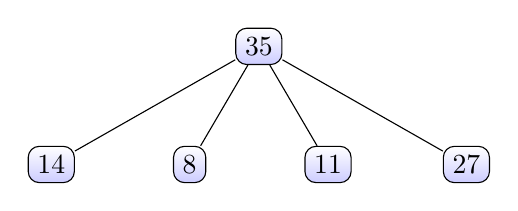
\begin{tikzpicture}[sibling distance=5em,
  every node/.style = {shape=rectangle, rounded corners,
    draw, align=center,
    top color=white, bottom color=blue!20}]]
  \node {35}
    child { node {14} }
    child { node {8} }
    child { node {11} }
    child { node {27} };
\end{tikzpicture}
\caption{Grafo de muestra del formato de un \textit{priority queue}.}
\end{figure}

El número 35 es el valor más alto y el que tiene la mayor prioridad, por lo tanto es el elemento al que se puede acceder. Ahora si ese valor se extrae, el \textit{priority queue} se reordena y queda de la siguiente forma:

\begin{figure}[h]
\centering
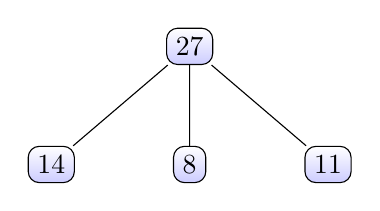
\begin{tikzpicture}[sibling distance=5em,
  every node/.style = {shape=rectangle, rounded corners,
    draw, align=center,
    top color=white, bottom color=blue!20}]]
  \node {27}
    child { node {14} }
    child { node {8} }
    child { node {11} };
\end{tikzpicture}
\caption{El \textit{priority queue} con el número 35 extraído.}
\end{figure}

En este caso el segundo valor más alto del \textit{priority queue} original (el número 27) es el nuevo elemento con la prioridad mayor y al que se puede acceder.

Ahora si se desea agregar un nuevo número a este arreglo, por ejemplo el 15, ocurre lo siguiente:

\begin{figure}[h]
\centering
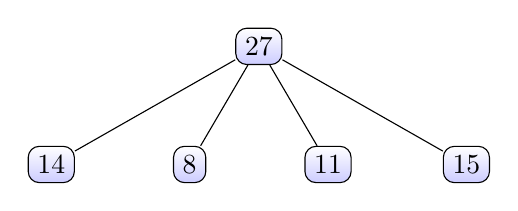
\begin{tikzpicture}[sibling distance=5em,
  every node/.style = {shape=rectangle, rounded corners,
    draw, align=center,
    top color=white, bottom color=blue!20}]]
  \node {27}
    child { node {14} }
    child { node {8} }
    child { node {11} }
    child { node {15} };
\end{tikzpicture}
\caption{El \textit{priority queue} con el número 15 agregado.}
\end{figure}

Como el número 15 es menor que 27, se mantiene este número como la mayor prioridad.

\subsection{Algunos comandos de C++ para el \textit{priority queue}}

En C++ se define como \texttt{priority\_queue<int>} ``nombre\_arreglo'' para guardar valores enteros, para este caso se definirá \texttt{mypq} como el nombre de ejemplo para esta estructura. Las operaciones más importantes que se pueden realizar para este tipo de estructura son las siguientes:

\begin{enumerate}

\item \texttt{mypq.push(n)}: Inserta el número $n$ en el \textit{priority queue}.
\item \texttt{mypq.top()}: Retorna el valor con mayor prioridad del \textit{priority queue}.
\item \texttt{mypq.pop()}: Remueve el valor con mayor prioridad del \textit{priority queue}, disminuyendo el largo de esta estructura en uno.
\item \texttt{mypq.empty()}: Retorna si el \textit{priority queue} está vacío.

\end{enumerate}

A partir de estas operaciones es posible manipular el \textit{priority queue} de manera más fácil, de tal manera que se usará esta estructura para guardar y obtener aquellos residuos de proteínas que más se repiten, sin embargo, para resolver el problema descrito será necesario guardar en este arreglo especial tanto el fragmento del péptido como la cantidad de repeticiones que posea, detalle que será visto en la sección de implementación.

\section{Restricciones para la propuesta}

Primero que todo, se extraerán las secuencias de polipéptidos de los archivos .fasta y se alinearán en una \textbf{única gran cadena} donde cada secuencia estará unida por un signo \$, con esto será posible identificar en los arreglos si cierto sufijo está compuesto por este signo o no, de esa forma descartarlo dentro de los diferentes residuos de aminoácidos que se cuentan:

\begin{table}[h]
\centering
\label{propuesta-22}
\begin{tabular}{c}
$\ldots$MPSTLQVLAKKVLKENDHISR\$EYHILKCWHEAPIILCFNGSKQM$\ldots$\\ 
\end{tabular}
\caption{2 secuencias enlazadas en una cadena general utilizando el signo \$ como unión.}
\end{table}

Para esta cadena grande (de largo $m$), el arreglo de sufijos y el arreglo LCP tendrán largo $m$, por lo cual para determinar los diferentes substrings de largo $k$ y aquellos substrings que más se repiten se debe recorrer el arreglo LCP completo, considerando:

\begin{enumerate}
\item Si el largo del sufijo es mayor o igual a $k$, entonces el arreglo LCP puede ser analizado, en caso contrario se omite y se continúa al siguiente valor del arreglo LCP.
\item Si el prefijo del sufijo revisado \textbf{solamente esté compuesto por los 20 aminoácidos conocidos} \cite{biomolecula}. Otros aminoácidos que no han sido definidos, como B, J, O, U o X serán omitidos para este problema (si son parte del substring del sufijo revisado, se omitirá y se continuará al arreglo LCP siguiente) y considerados como prohibidos \cite{aminoacids}. El signo \$ también será incluído a este grupo de carácteres prohibidos.
\end{enumerate}

Con respecto a esto es posible obtener los substrings diferentes y la cantidad de repeticiones que posee cada uno de estos, para posteriormente guardarlos en algun tipo de lista o vector. El problema es tratar de acceder a aquellos substrings que más se repiten, punto que se verá en la siguiente sección.

\section{Algoritmo desarrollado}

Para la obtención de los diferentes substrings se realizó un código implementado en lenguaje C++ \cite{tutorial} siguiendo varios puntos, en primera instancia para la base de datos de SwissProt, TrEMBL, EROP-Moscow y Proteínas Humanas se realizó una extracción previa de datos desde la página \texttt{http://www.uniprot.org/} (\cite{swissprot}, \cite{trembl}) y \texttt{http://erop.inbi.ras.ru/} \cite{eropmoscow} a comienzos de septiembre de este año. Para realizar esta preparación se aplicó un procedimiento en C++ para unir todas las cadenas de proteínas y generar una única cadena enlazada, cuya construcción será definida en la siguiente subsección.

\subsection{Extracción de proteínas desde el archivo .fasta}

Un archivo con el formato \textbf{.fasta} entrega cada polipéptido con un código o ID (que comienza con un $>$), a continuación en la misma línea se tiene al nombre taxativo de la proteína, y en la línea siguiente viene la cadena como tal, para luego repetir el proceso:

\begin{figure}[h]
    \centering
    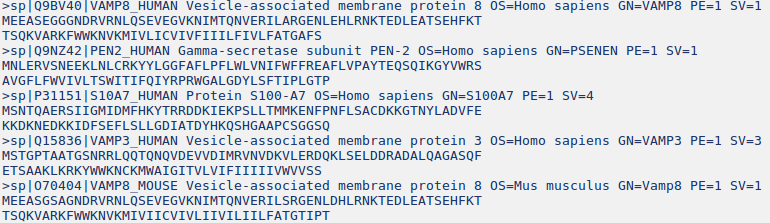
\includegraphics[width=0.9\textwidth]{./images/fastadefecto2.png}
    \caption{Archivo \textbf{.fasta} con varias proteínas}
    \label{fig:image5}
\end{figure}

Para extraer las cadenas se implementó el siguiente código en C++:

\begin{lstlisting}[language=C++, caption=Creación de cadena de proteínas.]
ifstream fin("uniprot_sprot.fasta"); //abrir archivo base
if(!fin){
	cerr << "Couldn't open the input file!";
	return(1);
}
ofstream outputfile; //crear archivo destino de cadena
outputfile.open("substrings.txt"); //definir nombre de archivo a crear
string line; 
int cantidad_ss = 1;

getline(fin, line); 
getline(fin, line); //tomar secuencia (1)

while(fin){
	if(line[0] == '>'){ // revisar primer elemento del string (2)
		outputfile << "$";
		cantidad_ss = cantidad_ss + 1;
	}
	else{
		outputfile << line;
	}
getline(fin, line); // continuar con la siguiente linea (3)
}

outputfile.close();
\end{lstlisting}

Lo que hace este código es crear un nuevo archivo ``substrings.txt'' en la variable \textbf{outputfile} donde se guardará la cadena de proteínas. Con \textit{getline} se lee la primera ĺinea del archivo .fasta que está guardada en la variable \textbf{fin}, e inmediatamente después se llama nuevamente a \textit{getline} para leer la segunda línea del archivo .fasta, que es \textbf{una secuencia o parte de ella} \textbf{(1)}. Luego se condiciona a realizar una de las 2 tareas siempre y cuando el archivo .fasta no se haya leído completamente: 

\begin{enumerate}
\item Si el primer elemento de la línea leída del archivo .fasta es $>$, significa que se llegó al final de una secuencia, por lo tanto es el comienzo de la siguiente (es la linea de definición de la proteína), en ese caso se le agrega el signo \$ al archivo destino como separador \textbf{(2)}. 
\item En caso contrario, se le agrega directamente la línea completa al archivo destino, ya que esta línea solamente está compuesta por \textbf{la secuencia en sí}.
\end{enumerate}

Finalmente se vuelve a llamar a \textit{getline} para continuar con la siguiente línea del archivo .fasta \textbf{(3)}.

En resumen el formato del nuevo archivo ``substrings.txt'' es una sola línea que tiene concatenada todas las proteínas:

\begin{table}[h]
\centering
\label{propuesta-23}
\begin{tabular}{c}
TSCPGGNHPVCCSTDLCNK\$MKTL$\ldots$SDLT\$LKCNKLVPLFYKTCP\\ 
\end{tabular}
\caption{Ejemplo de cadena encontrada en el archivo destino.}
\end{table}

Teniendo esta gran línea ya se puede construir el arreglo de sufijos y el arreglo LCP. Considerar como dato relevante que guardando esta cadena en una variable tipo \textit{string} cada caracter ocupa el largo de 1 byte de capacidad \cite{manipulatingstrings}, y esto determinará de qué manera se construirán los arreglos para la solución de este problema.

El largo de la cadena de proteínas generada de UniProt-SwissProt tiene un peso de 199 MB, mientras que para UniProt-TrEMBL su cadena de proteínas posee un peso de 30 GB, si separa EROP-Moscow el peso de su cadena de proteínas es de 0.35 MB y para las Proteínas Humanas la cadena generada tiene un tamaño de 38.2 MB.

Teniendo en consideración que para guardar la cadena en una variable ésta se almacena en la memoria RAM del ordenador. Se han realizado 2 implementaciones para la construcción de los arreglos.

\subsection{Implementación solución aplicando Memoria Interna}

Para la implementación del algoritmo se trabajó por medio del lenguaje C++ en base al algoritmo de Kasai \cite{kasaimethod}, \cite{kasai} para obtener el arreglo LCP en base al arreglo de sufijos. Antes que nada se define una estructura y una función comparativa que serán de soporte para la construcción del arreglo de sufijos:

\begin{lstlisting}[language=C++, caption=Definición previa de estructuras para construir el arreglo de sufijos.]
//  Struct para guardar la informacion de un sufijo
struct suffix
{
	int index; // Guardar el indice original
	int rank[2]; // Guarda los ranks y el rank pair siguiente
};

// Una funcion comparativa usada por sort () para comparar 2 sufijos
// Compara 2 pares, y retorna 1 si el primer par es mas pequeno
int cmp(struct suffix a, struct suffix b)
{
	return (a.rank[0] == b.rank[0])? (a.rank[1] < b.rank[1] ?1: 0):
		(a.rank[0] < b.rank[0] ?1: 0);
}
\end{lstlisting}

\textit{suffix} es una estructura que sirve para almacenar el índice original de determinado sufijo y los \textit{rank} donde se guardan los sufijos y su sufijo siguiente como pares. La función \textit{cmp} es usada para comparar entre los valores de los \textit{rank} entre 2 sufijos, y retorna 1 si el primer par es más pequeño, si son igual se continúa la comparación con el siguiente par, y es el comparador base que será usado por la función \textit{sort} más adelante.

\subsubsection{Arreglo de sufijos implementado}

Ahora se procederá a explicar la función principal que toma un string ``txt'' de largo n como entrada, y que construye y retorna el arreglo de sufijos para el string dado. Será explicado en secciones que fueron numerados en parte del código (con un //(número)) para aprovechar en mejor manera el formato de este documento:

\begin{lstlisting}[language=C++, caption=Función principal arreglo de sufijos (1).]
vector<int> buildSuffixArray(string txt, int n){

	struct suffix *suffixes = new struct suffix [n]; //(1)
	for (int i = 0; i < n; i++){
		suffixes[i].index = i;
		suffixes[i].rank[0] = txt[i] - 'a';
		suffixes[i].rank[1] = ((i+1) < n)? (txt[i + 1] - 'a'): -1;
	}
	sort(suffixes, suffixes+n, cmp); 
	int *ind = new int [n]; //(2)
	for (int k = 4; k < 2*n; k = k*2){
		int rank = 0;
		int prev_rank = suffixes[0].rank[0];
		suffixes[0].rank[0] = rank;
		ind[suffixes[0].index] = 0;//(3)
		for (int i = 1; i < n; i++){
			if (suffixes[i].rank[0] == prev_rank && 
			  suffixes[i].rank[1] == suffixes[i-1].rank[1]){ //(a)
				prev_rank = suffixes[i].rank[0];
				suffixes[i].rank[0] = rank;
			}
			else
			{
				prev_rank = suffixes[i].rank[0]; //(b)
				suffixes[i].rank[0] = ++rank;
			}
			ind[suffixes[i].index] = i;
		}
		for (int i = 0; i < n; i++){
			int nextindex = suffixes[i].index + k/2;
			suffixes[i].rank[1] = (nextindex < n)?
			    suffixes[ind[nextindex]].rank[0]: -1;
		}
		sort(suffixes, suffixes+n, cmp); //(4)
	}
	vector<int>suffixArr;
	for (int i = 0; i < n; i++){
        suffixArr.push_back(suffixes[i].index);
    } //(5)
	delete [] ind;
	delete [] suffixes;
	return suffixArr; //(6)
}

\end{lstlisting}

En \textbf{(1)} se crea un estructura que almacena sufijos y sus indices (\textit{suffixes}), que se alojará en memoria dinámica (operador new), esta estructura es necesaria para ordenar los sufijos de manera alfabética y mantener sus antiguos índices mientras se ordena. 

Luego con la función \textit{sort} se ordenan los sufijos de acuerdo a sus \textbf{2 primeros caracteres}. Una vez realizado esto de manera posterior se ordenan los sufijos de acuerdo a sus primeros 4 caracteres, luego con sus primeros 8 caracteres y asi sucesivamente hasta $k > 2^{n}$ donde $n$ es el largo del string analizado, para realizar esta tarea se crea un arreglo dinámico \textit{ind} que es necesario para obtener el indice original en la estructura suffixes[] \textbf{(2)}.

En cada una de estas iteraciones se le asigna los valores de \textit{rank} e índice al primer sufijo \textbf{(3)}, luego se le asigna los \textit{rank} a los siguientes sufijos hasta $n$ siguiendo ciertas reglas:

$a)$ Si el primer \textit{rank} y los siguientes ranks son iguales a aquellos de los sufijos anteriores en el arreglo, asignar el mismo nuevo rank a ese sufijo.\\
$b)$ En caso contrario aumentar el \textit{rank} y asignar.

Después se le asigna el próximo \textit{rank} a cada sufijo para posteriormente ordenar los sufijos según los primeros $k$ caracteres \textbf{(4)}. Se realiza este proceso hasta terminar las iteraciones para la variable $k$.

Finalmente en \textbf{(5)} se crea un vector que permita almacenar los valores obtenidos de los índices ordenados del arreglo \textit{suffixes}. Este vector de enteros \textit{suffixArr} se convertirá en el \textbf{arreglo de sufijos} del string \textit{txt}, luego se borran los arreglos dinámicos \textit{suffixes} e \textit{ind} para desocupar el espacio asignado en memoria RAM.

Posteriormente \textbf{(6)} se retorna el arreglo de sufijos final, que permitirá construir el arreglo LCP.

\subsubsection{Arreglo LCP implementado}

La implementación de este arreglo se hizo en base al \textit{suffix array} implementado, siguiendo lo descrito por Kasai \cite{kasaimethod}, \cite{kasai}. El código realizado es el siguiente:

\begin{lstlisting}[language=C++, caption=Función principal arreglo LCP (1).]
vector<int> lcp_str(string txt, vector<int> suffixArr){
	int n = suffixArr.size();
	vector<int> lcp(n, 0);
	vector<int> invSuff(n, 0); //(1)
	for (int i=0; i < n; i++)
		invSuff[suffixArr[i]] = i;

	int k = 0; //(2)
	for (int i=0; i<n; i++){
		if (invSuff[i] == n-1){
			k = 0;
			continue; //(3)
		}
		int j = suffixArr[invSuff[i]+1]; //(4)
		while (i+k<n && j+k<n && txt[i+k]==txt[j+k]) //(5)
			k++;
		lcp[invSuff[i]] = k; //(6)
		if (k>0)
			k--;
	}
	return lcp; //(7)
}

\end{lstlisting}

Lo que se hace en primera instancia es guardar el largo del arreglo, crear un vector para almacenar el arreglo LCP a construir y además crear un arreglo auxiliar $invSuff$ para almacenar el inverso del arreglo de sufijos previamente creado. Por ejemplo si $suffixArr[0]$ es 5, entonces $invSuff[5]$ debiese ser 0. Y esto será usado para obtener el siguiente string del arreglo de sufijos \textbf{(1)}.

Luego se llena con valores el arreglo $invSuff$ y se inicializa una variable para guardar la longitud del LCP del sufijo \textbf{(2)}. A partir de acá comienza a revisar todos los sufijos para asignarles su valor en el arreglo LCP.

Un detalle importante se ubica en \textbf{(3)}, ya que si el sufijo actual está ubicado en la posicion $n-1$, entonces ya no hay un siguiente substring a considerar, por lo tanto el LCP no es definido para este substring y se hace cero. Esto permitirá enfocar la solución del problema aumentando la cantidad de diferentes substrings desde 0 considerando determinados largos de LCPs consecutivos.

Posteriormente en la iteración se define una variable $j$ que contiene el índice del siguiente substring a ser considerado para compararlo con el actual substring, es decir, el siguiente string en el arreglo de sufijos \textbf{(4)}. Después la función \textit{while} comienza a revisar el sufijo desde el $k$-ésimo indice donde al menos $k-1$ caracteres serán similares, mientras esta condición se cumpla, $k$ va aumentando \textbf{(5)}.

Posteriormente se asigna el valor del LCP encontrado para el actual sufijo \textbf{(6)}, y $k$ se borra para utilizarlo en la siguiente iteración. Finalmente se retorma el arreglo LCP obtenido \textbf{(7)}.

Con esto se tienen a disposición los 2 arreglos necesarios como base para resolver el problema de la memoria.

\subsubsection{Implementación programa principal}

Ahora se procederá a explicar la implementación en la cual cómo se obtuvieron los diferentes substrings totales para cada $k$ entre 1 hasta 50 y la obtención de los residuos que más se repiten para cada caso. En primer lugar cuando la cadena de proteínas fue construída se definió una variable llamada \texttt{cantidad\_ss}, que guarda la cantidad total de proteínas analizadas. Utilizando las implementaciones del arreglo de sufijos y el arreglo LCP ocurre lo siguiente:

\begin{lstlisting}[language=C++, caption=Obtención de los arreglos SA y LCP para la cadena de proteínas.]
ifstream file("substrings.txt");
stringstream buffer;
buffer << file.rdbuf();
string str = buffer.str(); //(1)

unsigned t0, t1, t2, t3, t4, t5;
t0 = clock();
vector<int>suffixArr = buildSuffixArray(str, str.length());
t1 = clock();
double t12 = (double(t1-t0)/CLOCKS_PER_SEC); //(2)

t2 = clock();
vector<int>lcp = lcp_str(str, suffixArr);
t3 = clock();
double t23 = (double(t3-t2)/CLOCKS_PER_SEC); //(3)

ofstream resultados, k_utilizados; //(4)
resultados.open("resultados_sa_lcp.txt");
resultados << "Construccion SA: " << t12 << " segundos" << endl;
resultados << " \n";
resultados << "Construccion LCP: " << t23 << " segundos" << endl;
resultados << " \n";
resultados << "Total: " << cantidad_ss << " proteinas" << endl; //(5)
resultados.close();
	
\end{lstlisting}

En primera instancia se debe guardar la cadena de proteínas creada en el archivo ``substrings.txt'' en el string \texttt{str} \textbf{(1)}, para luego construir el arreglo de sufijos \textbf{(2)} que se guarda en el vector \texttt{suffixArr} y el arreglo LCP que se guarda en el vector \texttt{lcp} \textbf{(3)}. En ambos casos se obtienen los tiempos respectivos que demora en construir estos arreglos.

Después se crean 2 variables para crear archivos, en uno se guardarán los tiempos de construcción de los arreglos, y en otro los diferentes substrings para determinados $k$ con sus respectivos residuos que más se repiten \textbf{(4)}. A la primera variable se abre el archivo ``resultados\_sa\_lcp.txt'' y le agregan al archivo los tiempos de construcción de los 2 arreglos \textbf{(5)}, posteriormente este archivo se cierra.

El formato de los arreglos obtenidos es el siguiente:

\begin{table}[h]
\centering
\label{my-label15}
\begin{tabular}{llllllllllllll}
\cline{2-13}
\multicolumn{1}{l|}{Arreglo SA}  & \multicolumn{1}{l|}{...} & \multicolumn{1}{l|}{34} & \multicolumn{1}{l|}{22} & \multicolumn{1}{l|}{15} & \multicolumn{1}{l|}{89} & \multicolumn{1}{l|}{901} & \multicolumn{1}{l|}{1042} & \multicolumn{1}{l|}{45} & \multicolumn{1}{l|}{4} & \multicolumn{1}{l|}{47} & \multicolumn{1}{l|}{59} & \multicolumn{1}{l|}{...} &  \\ \cline{2-13}
                                 &                          &                         &                         &                         &                         &                          &                           &                         &                        &                         &                         &                          &  \\ \cline{2-13}
\multicolumn{1}{l|}{Arreglo LCP} & \multicolumn{1}{l|}{...} & \multicolumn{1}{l|}{2}  & \multicolumn{1}{l|}{0}  & \multicolumn{1}{l|}{21} & \multicolumn{1}{l|}{3}  & \multicolumn{1}{l|}{8}   & \multicolumn{1}{l|}{3}    & \multicolumn{1}{l|}{2}  & \multicolumn{1}{l|}{0} & \multicolumn{1}{l|}{0}  & \multicolumn{1}{l|}{9}  & \multicolumn{1}{l|}{...} &  \\ \cline{2-13}
\end{tabular}
\caption{Formatos de los arreglos SA y LCP.}
\end{table}

Recordar que todos los elementos del arreglo de sufijos son diferentes.

Para cada $k$ los arreglos se deben recorrer desde el principio hasta el final, con esto será posible obtener los diferentes residuos de péptidos y los que más se repiten. Esto se implementó de la siguiente forma:

\begin{lstlisting}[language=C++, caption=Obtención de los diferentes substrings de largo $k$ y los 20 substrings que más se repiten para la cadena de proteínas.]
int inicio = cantidad_ss - 1;
int n = suffixArr.size(); //(1)
k_utilizados.open("resultados_k1to50.txt");
for (int k1 = 1; k1 < 51; k1++){
    t4 = clock();
    subcadena arr[1];
    priority_queue<subcadena, vector<subcadena>, comparador> mypq; //(2)
    int activador = 0;
    int contador;
    int ds = 0; //(3)
    for (int temp = inicio; temp < n; temp++){ //(4)
        if (lcp[temp] >= k1 && activador == 0){ //(a)
            string sc = str.substr(suffixArr[temp], k1);
            if (sc.find_first_of("$BOUXZ")==std::string::npos){
                arr[0].nombre = sc;
                contador = 2;
                activador = 1;
            }
        }else if (lcp[temp] >= k1 && activador == 1){ //(b)
            string sc = str.substr(suffixArr[temp], k1);
            if (sc.find_first_of("$BOUXZ")==std::string::npos){
                contador = contador + 1;
            }else{
                arr[0].veces = contador;
                if (contador > 0){
                    mypq.push(arr[0]);
                }
                ds = ds + 1;
                activador = 0;
            }
        }else if (lcp[temp] < k1 && activador == 0){ //(c)
            string sc = str.substr(suffixArr[temp], k1);
            int scnumber = sc.size();
            if (scnumber == k1){
                if (sc.find_first_of("$BOUXZ")==std::string::npos){
                    ds = ds + 1;
                }
            }
        }else if (lcp[temp] < k1 && activador == 1){ //(d)
            arr[0].veces = contador;
            if (contador > 0){
                mypq.push(arr[0]);
            }
            ds = ds + 1;
            activador = 0;
        }
    }

    k_utilizados << "Diferentes residuos para " << k1 << " es " << ds << endl;
    k_utilizados << " \n";
    for (int posicion = 0; posicion < 20; posicion++){
        k_utilizados << mypq.top().nombre << " " << mypq.top().veces;
        mypq.pop();
        k_utilizados << endl; //(5)
    }
    t5 = clock();
    double t45 = (double(t5-t4)/CLOCKS_PER_SEC);
    k_utilizados << " \n"; 
    k_utilizados << "Tiempo utilizado: " << t45 << " segundos" << endl;
    k_utilizados << "--------------------------" << endl;
    k_utilizados << " \n";
}
k_utilizados.close(); //(6)
	
\end{lstlisting}

Lo primero que se hace es definir 2 variables, una (\texttt{n}) es para guardar el largo del arreglo de sufijos (que tiene el mismo largo que el arreglo LCP) y la otra variable (\texttt{inicio}) guarda el total de proteínas analizadas menos una unidad, que será usada en las iteraciones \textbf{(1)}. Luego se abre el archivo ``resultados\_k1to50.txt'' y se deja así hasta que la iteración completa termine, ya que en este archivo se guardarán los resultados obtenidos con el algoritmo.

La iteración principal abarcará desde $k=1$ hasta 50, es decir que para cada $k$ se recorrerán los arreglos desde principio a fin. Una vez definido $k$ se crea un arreglo \texttt{arr[1]} y el posterior \textit{priority queue} que está creado en base a una estructura llamada \texttt{subcadena} y una clase llamada \texttt{comparador}:

\begin{lstlisting}[language=C++, caption=Implementación de \texttt{subcadena} y \texttt{comparador} como soportes del \textit{priority queue} a utilizar.]
struct subcadena
{
  string nombre;
  int veces;
};

class comparador
{
 public:
   bool operator()(const subcadena& a, const subcadena& b)
   {
        return a.veces<b.veces;
   }
};	
\end{lstlisting}

Esta estructura permitirá guardar la cadena de substring y la cantidad de veces que aparezca en la cadena de proteínas, mientras que la clase es usada para comparar entre los substrings agregados al \textit{priority queue} y retornar cuál de ellos \textbf{tiene el valor más alto}, gracias a esto es posible obtener cuál es el substring que más se repite y su cantidad \textbf{(2)}.

Antes de iterar sobre los arreglos, se definen 3 variables importantes \textbf{(3)}, que son:

\begin{enumerate}

\item \texttt{activador}: Esta variable es usada para verificar si se están sumando repeticiones de un determinado residuo o no. Toma valores entre 0 y 1, donde 0 significa que se están buscando substrings y 1 significa que se están agregando repeticiones de determinado substring encontrado. Esto está asociado directamente con el arreglo creado \texttt{arr}, si se guarda en este arreglo solamente el substring y continuan las iteraciones, \texttt{activador} toma el valor 1 y si se guarda la cantidad de repeticiones en el arreglo \texttt{arr}, \texttt{activador} toma el valor 0.
\item \texttt{contador}: Esta variable es usada para guardar la cantidad de repeticiones de un determinado residuo.
\item \texttt{ds}: Esta variable guarda la cantidad de diferentes substrings encontrados de largo $k$.
\end{enumerate}

Con esto definido se puede comenzar a iterar sobre los arreglos. La primera posición denominada como \texttt{inicio} está ubicada en \texttt{cantidad\_ss-1} ya que a cada proteína se le concatena con el signo \$, por lo tanto si se concatenan $N$ proteínas de un archivo .fasta, se tienen en total $N$ veces el signo \$, y considerando que el arreglo de sufijos ordena cada sufijo según su orden alfabético, este signo se ubica antes de la letra $a$ y además se tiene que este signo pertenece a los carácteres prohibidos, por consiguiente no es necesario revisar estos sufijos \textbf{(4)}.

Ahora se comienza a iterar sobre el arreglo LCP (variable \texttt{temp} que indica la posición en el arreglo), verificando si el valor es mayor o igual a $k$. Ante esto se tienen 4 casos que se pueden formar:  

$a)$ Si \texttt{lcp[temp]} $>= k$ y \texttt{activador} $= 0$: Si esto ocurre \textbf{(a)} se guarda el substring que corresponde al residuo de proteínas en la posición \texttt{temp} de largo $k$ (\texttt{substr(suffixArr[temp], k)}) y se revisa si este substring posee alguno de los caracteres prohibidos, en caso negativo se guarda este residuo en la estructura \texttt{arr} y se inicializa \texttt{contador} con un valor de 2, porque acá se tienen al menos \textbf{2 repeticiones} del substring hallado y \texttt{activador} toma el valor de 1 ya que comienza la búsqueda de más repeticiones del substring encontrado; en caso afirmativo se continúa con la siguiente iteración del arreglo.

\begin{figure}[h]
\centering
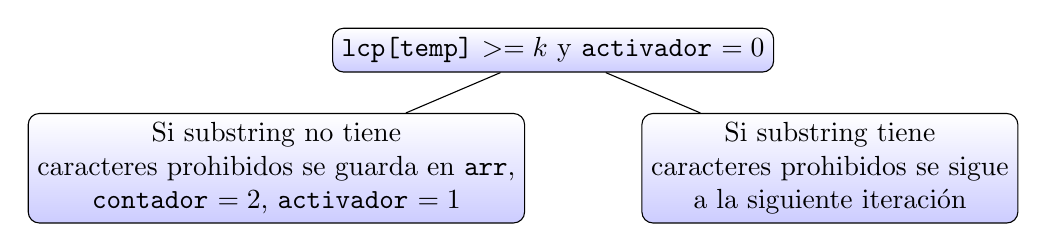
\begin{tikzpicture}[sibling distance=20em, level distance=1.5cm,
  every node/.style = {shape=rectangle, rounded corners,
    draw, align=center,
    top color=white, bottom color=blue!20}]]
  \node {\texttt{lcp[temp]} $>= k$ y \texttt{activador} $= 0$}
    child { node {Si substring no tiene\\caracteres prohibidos se guarda en \texttt{arr},\\\texttt{contador} $= 2$, \texttt{activador} $= 1$} }
    child { node {Si substring tiene\\caracteres prohibidos se sigue\\a la siguiente iteración} };
\end{tikzpicture}
\caption{Esquema Caso $a)$.}
\end{figure}

$b)$ Si \texttt{lcp[temp]} $>= k$ y \texttt{activador} $= 1$: Si este caso pasa ahora se deberá comparar el sufijo de esta posición \texttt{temp} cumple con la condición de no tener caracteres prohibidos \textbf{(b)}, si la cumple a \texttt{contador} se le debe adicionar una unidad; si esto no se cumple es decir que se acabaron las repeticiones para el substring y se guarda en la estructura \texttt{arr} la cantidad de repeticiones obtenidas hasta ese momento para el substring previamente guardado en esa estructura, para después guardar el substring y sus repeticiones en forma de nodo en el \textit{priority queue}, y posteriormente agregarle una unidad a la variable \texttt{ds} (de diferentes substrings) ya que el substring anterior no se volverá a encontrar en el arreglo de sufijos, finalmente la variable \texttt{activador} se hace 0.

\begin{figure}[h]
\centering
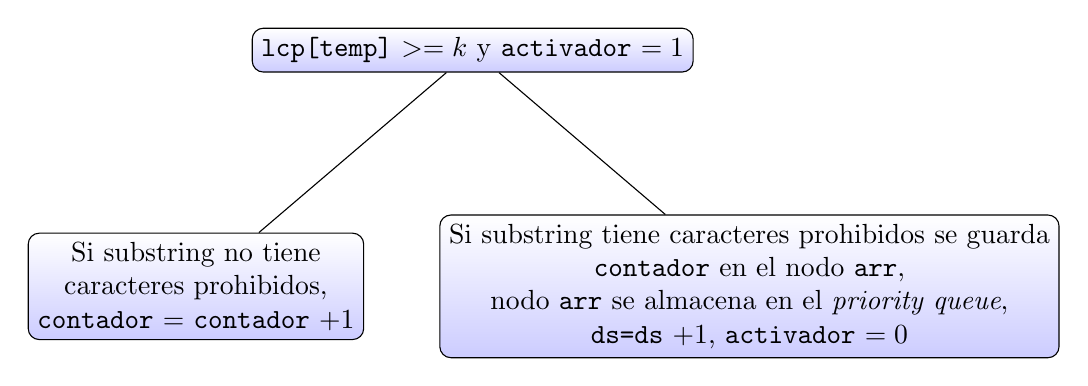
\begin{tikzpicture}[sibling distance=20em, level distance=3cm,
  every node/.style = {shape=rectangle, rounded corners,
    draw, align=center,
    top color=white, bottom color=blue!20}]]
  \node {\texttt{lcp[temp]} $>= k$ y \texttt{activador} $= 1$}
    child { node {Si substring no tiene\\caracteres prohibidos,\\\texttt{contador} $=$ \texttt{contador} $+ 1$} }
    child { node {Si substring tiene caracteres prohibidos se guarda \\\texttt{contador} en el nodo \texttt{arr}, \\nodo \texttt{arr} se almacena en el \textit{priority queue},\\\texttt{ds=ds} $+ 1$, \texttt{activador} $= 0$} };
\end{tikzpicture}
\caption{Esquema Caso $b)$.}
\end{figure}

$c)$ Si \texttt{lcp[temp]} $< k$ y \texttt{activador} $= 0$: Como el valor del arreglo LCP en la posición \texttt{temp} es menor que $k$ acá simplemente se verifica que el substring de largo $k$ correspondiente a la posición \texttt{temp} en el arreglo de sufijos tenga un largo igual a $k$  y que no tenga caracteres prohibidos \textbf{(c)}, si no tiene entonces a la variable \texttt{ds} se le agrega una unidad y se guarda el substring con el valor 1 con forma de nodo en el \textit{priority queue}.

\begin{figure}[h]
\centering
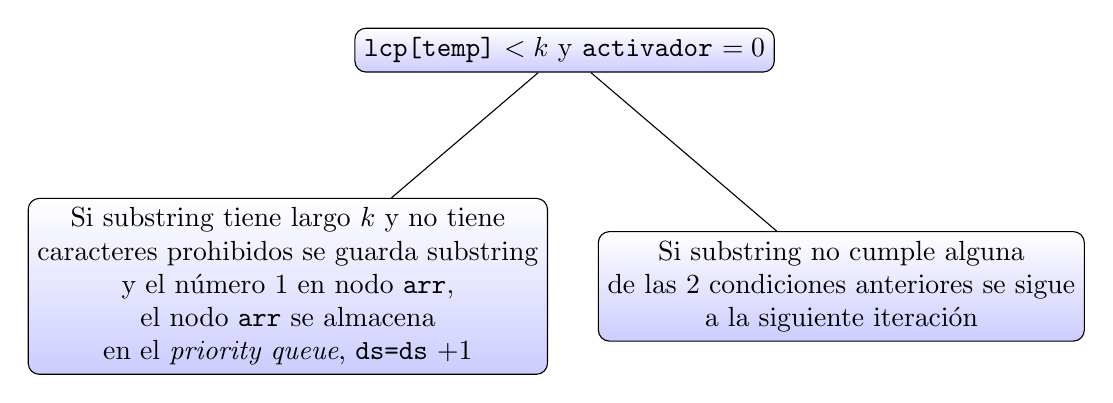
\begin{tikzpicture}[sibling distance=20em, level distance=3cm,
  every node/.style = {shape=rectangle, rounded corners,
    draw, align=center,
    top color=white, bottom color=blue!20}]]
  \node {\texttt{lcp[temp]} $< k$ y \texttt{activador} $= 0$}
    child { node {Si substring tiene largo $k$ y no tiene\\caracteres prohibidos se guarda substring\\y el número 1 en nodo \texttt{arr},\\el nodo \texttt{arr} se almacena\\en el \textit{priority queue}, \texttt{ds=ds} $+ 1$} }
    child { node {Si substring no cumple alguna\\de las 2 condiciones anteriores se sigue\\a la siguiente iteración} };
\end{tikzpicture}
\caption{Esquema Caso $c)$.}
\end{figure}

$d)$ Si \texttt{lcp[temp]} $< k$ y \texttt{activador} $= 1$: Acá ya se tiene guardado un substring en el arreglo \texttt{arr} porque el activador está con valor 1, por ende el arreglo LCP actual es menor al $k$ requerido \textbf{(d)} y se guarda la variable \texttt{contador} en el arreglo \texttt{arr} para luego almacenar esta variable como nodo en el \textit{priority queue}, se le agrega una unidad a la variable \texttt{ds} y la variable \texttt{activador} se hace 0.

\begin{figure}[h]
\centering
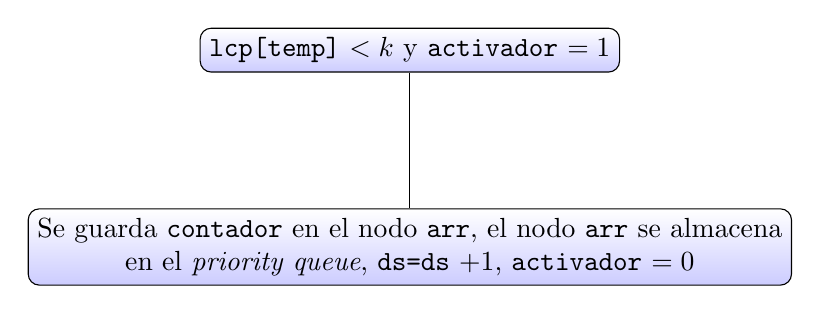
\begin{tikzpicture}[sibling distance=20em, level distance=2.5cm,
  every node/.style = {shape=rectangle, rounded corners,
    draw, align=center,
    top color=white, bottom color=blue!20}]]
  \node {\texttt{lcp[temp]} $< k$ y \texttt{activador} $= 1$}
    child { node {Se guarda \texttt{contador} en el nodo \texttt{arr}, el nodo \texttt{arr} se almacena\\en el \textit{priority queue}, \texttt{ds=ds} $+ 1$, \texttt{activador} $= 0$} };
\end{tikzpicture}
\caption{Esquema Caso $d)$.}
\end{figure}

Una vez recorrido el arreglo se guarda en el archivo destino (``resultados\_k1to50.txt'') los diferentes substrings obtenidos (\texttt{ds}) y luego utilizando los comandos explicados anteriormente sobre el \textit{priority queue} se extraen los \textbf{20 primeros residuos de proteínas que más se repiten junto a su cantidad total} y se guardan en este archivo \textbf{(5)}, y luego se reinicia la iteración principal con el siguiente $k$ a utilizar.

Una vez usados todos los $k$ permitidos \textbf{(6)} se cierra el archivo destino y se termina de ejecutar el archivo.

\subsubsection{Formato salida archivos}

Después de haber ejecutado este algoritmo se obtiene el archivo de salida mencionado anteriormente, llamado ``resultados\_k1to50.txt'' y que tiene el siguiente formato:

\begin{figure}[h]
    \centering
    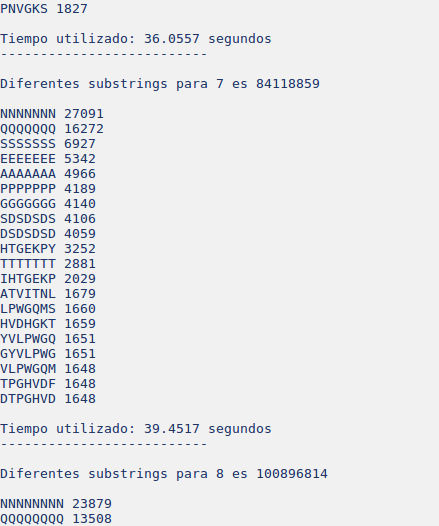
\includegraphics[width=0.5\textwidth]{./images/formatosalidaswissprot.png}
    \caption{Extracto del archivo de salida ``resultados\_k1to50.txt''.}
\end{figure}

Como se puede apreciar en la imagen, se han guardado las cantidades de diferentes substrings obtenidos para cada $k$ (en la imagen se muestra para $k = 7$), los 20 residuos que más repiten con su respectiva cantidad de repeticiones encontradas y el tiempo en recorrer los arreglos para determinado $k$. Las líneas salteadas indican el cambio hacia el siguiente $k$ (para la imagen es $k=8$) nuevamente mostrando los diferentes substrings encontrados y los 20 residuos que más se repiten. Este proceso inicia con $k=1$ hasta llegar a $k=50$.

\subsection{Implementación solución aplicando Memoria Externa}

Para archivos muy grandes que superen los 1000 MB de capacidad como la base de datos UniProt-TrEMBL es inviable guardar los arreglos (tanto de sufijos como LCP) en memoria RAM ya que el espacio requerido no es el suficiente ($9n$ donde $n$ es el tamaño de bytes de la cadena de strings). Ante esa problemática se procedió a buscar una alternativa para trabajar este gran archivo.

En el intertanto de la búsqueda de opciones, se descubrió que existen algoritmos que desarrollan arreglos de sufijos de archivos cuyos tamaños eran superiores a la memoria RAM corriente (computadores de hasta 8 GB de capacidad) y dentro de esas alternativas se decidió trabajar con algoritmos en memoria externa.

La implementación realizada se hizo en lenguaje C++ en base al trabajo e investigación efectuada por Juha Kärkkäinen y Dominik Kempa (\cite{sascan}, \cite{emsparse}) para obtener el arreglo de sufijos y el arreglo LCP en memoria externa. Ambos casos usan un archivo MAKEFILE para ejecutar las implementaciones, en consecuencia para cada uno de estos casos se explicarán los pasos más relevantes que permiten obtener los arreglos como resultado final.

\subsubsection{Arreglo de sufijos EM implementado}

Tomando la cadena de proteínas, lo primero que se hace es particionar el string en bloques más pequeños, lo suficiente para que puedan ser analizados en memoria RAM. Luego para cada bloque se construye el arreglo de sufijos utilizando una librería de ordenamiento llamada ``libdivsufsort'' \cite{yutamori} y estos se guardan en el disco duro.

Las combinaciones de los arreglos se realizan desde el último bloque hasta el bloque inicial, considerando la siguiente idea:

Se combinan 2 bloques X e Y en el cual $SA_{Y}$ es el arreglo de sufijos del texto Y, y para el texto X se construye el arreglo de sufijos parcial $SA_{X:Y}$ el cual posee los sufijos de XY pero solamente considerando posiciones iniciales en el texto X. Como ejemplo explicativo se tomará la palabra BANANA la cual se particionará en 2 bloques:

\begin{table}[h]
\centering
\begin{tabular}{cccccccccccccc}
0                       & 1                      & 2                      & 3                      & 4                      & 5                      &                                    & 0                      & 1                      & 2                      &                       & 0                      & 1                      & 2                      \\ \cline{1-6} \cline{8-10} \cline{12-14} 
\multicolumn{1}{|c|}{B} & \multicolumn{1}{c|}{A} & \multicolumn{1}{c|}{N} & \multicolumn{1}{c|}{A} & \multicolumn{1}{c|}{N} & \multicolumn{1}{c|}{A} & \multicolumn{1}{c|}{$->$} & \multicolumn{1}{c|}{B} & \multicolumn{1}{c|}{A} & \multicolumn{1}{c|}{N} & \multicolumn{1}{c|}{} & \multicolumn{1}{c|}{A} & \multicolumn{1}{c|}{N} & \multicolumn{1}{c|}{A} \\ \cline{1-6} \cline{8-10} \cline{12-14} 
\end{tabular}
\caption{Partición de la palabra BANANA en 2 bloques de texto}
\end{table}

Los arreglos de sufijos formados según la explicación anterior para estos bloques son los siguientes:

\newpage

\begin{table}[h]
\centering
\begin{tabular}{cccccccccc}
\cline{3-3}
                   & \multicolumn{1}{c|}{} & \multicolumn{1}{c|}{1} & A & N & $|$ & A & N & A &   \\ \cline{3-3}
X $->$ \texttt{SA\textsubscript{X:Y}} & \multicolumn{1}{c|}{} & \multicolumn{1}{c|}{0} & B & A & N & $|$ & A & N & A \\ \cline{3-3}
                   & \multicolumn{1}{c|}{} & \multicolumn{1}{c|}{2} & N & $|$ & A & N & A &   &   \\ \cline{3-3}
                   &                       &                        &   &   &   &   &   &   &   \\ \cline{3-3}
                   & \multicolumn{1}{c|}{} & \multicolumn{1}{c|}{2} & A &   &   &   &   &   &   \\ \cline{3-3}
Y $->$ \texttt{SA\textsubscript{Y}} & \multicolumn{1}{c|}{} & \multicolumn{1}{c|}{0} & A & N & A &   &   &   &   \\ \cline{3-3}
                   & \multicolumn{1}{c|}{} & \multicolumn{1}{c|}{1} & N & A &   &   &   &   &   \\ \cline{3-3}
\end{tabular}
\caption{Arreglos de sufijos formados de los bloques de textos.}
\end{table}

Estos bloques se almacenan en disco duro y para combinarlos, se utiliza un arreglo de espacios (\textit{gap array}) donde \texttt{gap\textsubscript{X:Y}[i]} es el número de sufijos de Y que lexicográficamente se ubican entre los sufijos \texttt{SA\textsubscript{X:Y}[i-1]} y \texttt{SA\textsubscript{X:Y}[i]} de XY. Volviendo a la palabra BANANA, este arreglo de espacio se construye de la siguiente forma:

\begin{enumerate}

\item Sufijos lexicográficamente menores que ANANA que están en Y: 2 (A y ANA).
\item Sufijos ubicados lexicográficamente entre ANANA y BANANA que están en Y: 0.
\item Sufijos ubicados lexicográficamente entre BANANA y NANA que están en Y: 1 (NA).
\item Sufijos lexicográficamente mayores que NANA que están en Y: 0.

\end{enumerate}

Por consiguiente el arreglo \texttt{gap\textsubscript{X:Y}} estaría compuesto de la siguiente forma:

\begin{table}[!hbt]
\centering
\begin{tabular}{|l|l|l|l|}
\hline
2 & 0 & 1 & 0 \\ \hline
\end{tabular}
\caption{Arreglo de espacios generado de los arreglos de sufijos anteriormente obtenidos.}
\end{table} 

Con estos 3 arreglos ya es posible efectuar la combinación, considerando un arreglo vacío cuyo largo son las sumas de los largos de los arreglos de sufijos \texttt{SA\textsubscript{X:Y}} y \texttt{SA\textsubscript{Y}}. Para comenzar a insertarle números se utilizan primero los elementos del arreglo \texttt{SA\textsubscript{X:Y}} utilizando el arreglo \texttt{gap\textsubscript{X:Y}} como soporte de posiciones. Luego se insertan los elementos del arreglo \texttt{SA\textsubscript{Y}} adicionándole a cada elemento en forma de unidades el largo del arreglo \texttt{SA\textsubscript{X:Y}}. Se puede ejemplificar mejor si se utiliza la palabra BANANA. Primero que todo se tiene el arreglo combinatorio \texttt{SA\textsubscript{XY}} vacío:

\begin{table}[!hbt]
\centering
\begin{tabular}{cc|c|c|c|c|c|c|}
\cline{3-8}
\texttt{SA\textsubscript{XY}} &  $->$ &  &  &  &  &  &  \\ \cline{3-8} 
\end{tabular}
\caption{Arreglo de sufijos XY vacío.}
\end{table}

\newpage

$a)$ Colocarse en \texttt{SA\textsubscript{XY}[0]}, e insertar elemento \texttt{SA\textsubscript{X:Y}[0]} $= 1$ en el arreglo, pero como \texttt{gap\textsubscript{X:Y}[0]} $= 2$, se avanzan 2 posiciones en el arreglo combinado y se inserta el elemento en \texttt{SA\textsubscript{XY}[2]}:

\begin{table}[!hbt]
\centering
\begin{tabular}{cc|c|c|c|c|c|c|}
\cline{3-8}
\texttt{SA\textsubscript{XY}} &  $->$ &  &  & 1 &  &  &  \\ \cline{3-8} 
\end{tabular}
\caption{Arreglo de sufijos XY primer elemento insertado.}
\end{table}

$b)$ Avanzar y colocarse en \texttt{SA\textsubscript{XY}[3]}, e insertar elemento \texttt{SA\textsubscript{X:Y}[1]} $= 0$ en el arreglo, como \texttt{gap\textsubscript{X:Y}[1]} $= 0$, no se avanzan posiciones en el arreglo combinado y se inserta el elemento en \texttt{SA\textsubscript{XY}[3]}:

\begin{table}[!hbt]
\centering
\begin{tabular}{cc|c|c|c|c|c|c|}
\cline{3-8}
\texttt{SA\textsubscript{XY}} &  $->$ &  &  & 1 & 0 &  &  \\ \cline{3-8} 
\end{tabular}
\caption{Arreglo de sufijos XY segundo elemento insertado.}
\end{table}

$c)$ Avanzar y colocarse en \texttt{SA\textsubscript{XY}[4]}, e insertar elemento \texttt{SA\textsubscript{X:Y}[2]} $= 2$ en el arreglo, pero como \texttt{gap\textsubscript{X:Y}[2]} $= 1$, se avanza 1 posición en el arreglo combinado y se inserta el elemento en \texttt{SA\textsubscript{XY}[5]}:

\begin{table}[!hbt]
\centering
\begin{tabular}{cc|c|c|c|c|c|c|}
\cline{3-8}
\texttt{SA\textsubscript{XY}} &  $->$ &  &  & 1 & 0 &  & 2 \\ \cline{3-8} 
\end{tabular}
\caption{Arreglo de sufijos XY tercer elemento insertado.}
\end{table}

Como ya se insertaron todos los elementos del arreglo de sufijos X:Y, ya no será necesario utilizar el arreglo \texttt{gap\textsubscript{X:Y}}. Ahora se deben insertar los elementos del arreglo \texttt{SA\textsubscript{Y}} regresando a la primera posición vacía del arreglo combinado.

$d)$ Colocarse en \texttt{SA\textsubscript{XY}[0]} (primer espacio vacío disponible), e insertar elemento \texttt{SA\textsubscript{Y}[0]} $= 2$ en el arreglo, agregándole 3 unidades por el largo del arreglo \texttt{SA\textsubscript{X:Y}}:

\begin{table}[!hbt]
\centering
\begin{tabular}{cc|c|c|c|c|c|c|}
\cline{3-8}
\texttt{SA\textsubscript{XY}} &  $->$ & 5 &  & 1 & 0 &  & 2 \\ \cline{3-8} 
\end{tabular}
\caption{Arreglo de sufijos XY cuarto elemento insertado.}
\end{table}

$e)$ Avanzar y colocarse en \texttt{SA\textsubscript{XY}[1]} (primer espacio vacío disponible), e insertar elemento \texttt{SA\textsubscript{Y}[1]} $= 0$ en el arreglo, agregándole 3 unidades por el largo del arreglo \texttt{SA\textsubscript{X:Y}}:

\begin{table}[!hbt]
\centering
\begin{tabular}{cc|c|c|c|c|c|c|}
\cline{3-8}
\texttt{SA\textsubscript{XY}} &  $->$ & 5 & 3 & 1 & 0 &  & 2 \\ \cline{3-8} 
\end{tabular}
\caption{Arreglo de sufijos XY quinto elemento insertado.}
\end{table}

$f)$ Avanzar y colocarse en \texttt{SA\textsubscript{XY}[4]} (primer espacio vacío disponible), e insertar elemento \texttt{SA\textsubscript{Y}[2]} $= 1$ en el arreglo, agregándole 3 unidades por el largo del arreglo \texttt{SA\textsubscript{X:Y}}:

\newpage

\begin{table}[!hbt]
\centering
\begin{tabular}{cc|c|c|c|c|c|c|}
\cline{3-8}
\texttt{SA\textsubscript{XY}} &  $->$ & 5 & 3 & 1 & 0 & 4 & 2 \\ \cline{3-8} 
\end{tabular}
\caption{Arreglo de sufijos XY todos los elementos insertado.}
\end{table}

Y así quedaría el arreglo de sufijos final para XY. Se puede verificar si el arreglo de sufijos obtenido para BANANA está correcto:

\begin{table}[!hbt]
\centering
\begin{tabular}{cccccc}
\hline
\multicolumn{1}{|c|}{5} & \multicolumn{1}{c|}{3} & \multicolumn{1}{c|}{1} & \multicolumn{1}{c|}{0} & \multicolumn{1}{c|}{4} & \multicolumn{1}{c|}{2} \\ \hline
A                       & A                      & A                      & B                      & N                      & N                      \\
                        & N                      & N                      & A                      & A                      & A                      \\
                        & A                      & A                      & N                      &                        & N                      \\
                        &                        & N                      & A                      &                        & A                      \\
                        &                        & A                      & N                      &                        &                        \\
                        &                        &                        & A                      &                        &                       
\end{tabular}
\caption{Arreglo de sufijos de la palabra BANANA.}
\end{table}

Con esto se corrobora que el método explicado es el adecuado. Si se tuvieran más de 2 bloques se continúan formando arreglos de sufijos parciales \texttt{SA\textsubscript{X:Y}} con los nuevos textos X y los bloques combinados Y generados en los pasos anteriores. Estos bloques se van alojando en el disco duro, entregando una complejidad I/O (escritura y lectura) muy alta hasta formar el arreglo de sufijos definitivo, que es guardado también en disco duro ya que será utilizado para la construcción del arreglo LCP en memoria externa. Guardar este archivo considera un uso de disco duro de $5n$ bytes (considerando que el texto o cadena pesa $n$ bytes). Acceder a este archivo (formato .sa5) de manera convencional no es posible, es necesario llevar los datos a un archivo .txt para trabajarlos más fácilmente. Este punto será visto con mayor detalle en la próxima parte, los arreglos LCP en memoria externa. 

La implementación a nivel de código es bien compleja y díficil de explicar (realizada por los investigadores anteriormente nombrados, que tienen muchos archivos con código que se relacionan entre sí) por lo mismo se decidió mencionar en grandes rasgos cuáles son las etapas más importantes de este algoritmo. Para generar este arreglo de sufijos en memoria externa los investigadores usaron técnicas como la Transformación de Burrows-Wheeler y algunas estructuras de soporte que permiten leer y escribir en estos archivos.

\subsubsection{Arreglo LCP EM implementado}

Para construir este arreglo es necesario recibir como \textit{input} el texto (cadena) de largo $n$ y el arreglo de sufijos previamente construído y guardado en disco duro. Se realizan 3 pasos importantes en la implementación:

$a)$ Por medio del arreglo de sufijos, construir un arreglo $\Phi_{q}$ utilizando un $q$ de tal manera que el arreglo permutado \texttt{PLCP\textsubscript{q}} pueda caber en la memoria RAM.

Se mencionó en la sección del Estado del Arte que el arreglo $\Phi$ es un arreglo cuya propiedad es que $\Phi[i]$ guarda el predecesor inmediato del sufijo $i$ ($\Phi[SA[j]]$ $=$ $SA[j-1]$) y obteniendo los valores lcp($i$, $\Phi[i]$) para todo $i \in [0,n-1]$ es posible de construir este arreglo PLCP. Ahora bien, si este arreglo se evalúa utilizando los $SA[i]$ obtenidos anteriormente, se tiene el arreglo LCP final, pero este arreglo no va a caber completamente en la memoria RAM, por lo mismo es que se utiliza un $q \geq 1$ para limitar el tamaño de los arreglos $\Phi$ y PLCP. Se usará el ejemplo anterior de BANANA, ya que se tiene su arreglo de sufijos listo.

\begin{table}[!htb]
\centering
\begin{tabular}{|c|c|c|c|c|c|}
\hline
5 & 3 & 1 & 0 & 4 & 2 \\ \hline
\end{tabular}
\caption{Arreglo de sufijos de la palabra BANANA.}
\end{table}

El $q$ a utilizar será 2 lo que permitirá disminuir el tamaño del arreglo $\Phi$ original a la mitad (6 $->$ $\left \lceil{6/2}\right \rceil$ 3) lo que conllevará a obtener una representación compacta del arreglo PLCP (de tamaño 3 también) a posterior.

Para obtener los valores de este arreglo $\Phi_{2}$ se debe recorrer el arreglo de sufijos y de esa manera identificar usando $i \in [1,n]$ si los residuos generados de la división entre $SA[i]$ y $q=2$ son nulos ($SA[i]$ mod $2 = 0$). En caso afirmativo se agregará un valor al arreglo $\Phi_{2}$ que será el sufijo anterior $SA[i-1]$, en caso contrario seguirá con la siguiente iteración. Entonces para BANANA se tiene que:

\begin{enumerate}

\item $i = 1: SA[1]$ mod $2 = 1 (3/2) \rightarrow$ No sirve.
\item $i = 2: SA[2]$ mod $2 = 1 (1/2) \rightarrow$ No sirve.
\item $i = 3: SA[3]$ mod $2 = 0 (0/2) \rightarrow \Phi_{2}[SA[3]/2] \rightarrow \Phi_{2}[0/2] \rightarrow \Phi_{2}[0]\rightarrow SA[2] = 1$.

\begin{table}[!htb]
\centering
\begin{tabular}{c|c|c|c|}
\cline{2-4}
$\Phi_{2}[i]:$ & 1 &  & \\ \cline{2-4}
\end{tabular}
\caption{Arreglo $\Phi_{2}$ con el primer elemento agregado.}
\end{table}

\item $i = 4: SA[4]$ mod $2 = 0 (4/2) \rightarrow \Phi_{2}[SA[4]/2] \rightarrow \Phi_{2}[4/2] \rightarrow \Phi_{2}[2] \rightarrow SA[3] = 0$.

\begin{table}[!htb]
\centering
\begin{tabular}{c|c|c|c|}
\cline{2-4}
$\Phi_{2}[i]:$ & 1 &  & 0\\ \cline{2-4}
\end{tabular}
\caption{Arreglo $\Phi_{2}$ con el segundo elemento agregado.}
\end{table}

\item $i = 5: SA[5]$ mod $2 = 0 (2/2) \rightarrow \Phi_{2}[SA[5]/2] \rightarrow \Phi_{2}[2/2] \rightarrow \Phi_{2}[1] \rightarrow SA[4] = 4$.

\begin{table}[!htb]
\centering
\begin{tabular}{c|c|c|c|}
\cline{2-4}
$\Phi_{2}[i]:$ & 1 & 4 & 0\\ \cline{2-4}
\end{tabular}
\caption{Arreglo $\Phi_{2}$ con todos los elementos agregados.}
\end{table}

\item $i = 6: SA[6]$ mod $2 =$ indeterminado porque $SA[6]$ no tiene valor.

\end{enumerate}

\newpage

Por lo tanto el arreglo $\Phi_{2}$ se ordena dependiendo de $q$:

\begin{table}[!htb]
\centering
\begin{tabular}{c|c|c|c|c|c|c|cc|c|c|c|}
\cline{2-7} \cline{10-12}
$SA[i]$: & 5 & 3 & 1 & 0 & 4 & 2 &  & $\Phi_{2}[i]$: & 1 & 4 & 0 \\ \cline{2-7} \cline{10-12} 
\end{tabular}
\caption{Arreglo de sufijos y arreglo $\Phi_{2}$ de la palabra BANANA.}
\end{table}


Este arreglo $\Phi_{q}$ o sus elementos conocidos como el par ($i$, $\Phi_{q}[i]$) se guardan en disco duro. En el caso de que el texto tengo un tamaño mayor a la memoria RAM permitida el texto se particiona en bloques y sus pares ($i$, $\Phi_{q}[i]$) se van guardando en un archivo asociado con el segmento de texto que contenga a $\Phi_{q}[i]$.

$b)$ Utilizando el arreglo $\Phi_{q}$ creado y la cadena de texto $T$ obtener el arreglo $PLCP_{q}$.

Para construir este arreglo se inicializa la variable $l=0$ y será necesario realizar una serie de comparaciones de las posiciones de los caracteres de la cadena que es T[$j \times 2+l$] $=$ T[$\Phi_{2}[i]+l$] utilizando el par ($j$, $\Phi_{2}[j]$) para $j \in [0, \left \lceil{6/2}\right \rceil - 1]$. Cada vez que se cumpla la comparación se aumentará en una unidad el valor de la variable $l$ y se volverá a realizar la comparación hasta que haya una desigualdad y de esa forma salir del bucle. Esta variable $l$ es la que permitirá guardar los valores en el arreglo $PLCP_{2}$.

\begin{enumerate}

\item $j=0: l=0 \rightarrow$ T[$0 \times 2+0$] $=$ T[$1+0$] $\rightarrow$ T[$0$] $=$ T[$1$] $\rightarrow$ B $\neq$ A $\therefore l=0 \rightarrow PLCP_{2}[0] = 0$.

\begin{table}[!htb]
\centering
\begin{tabular}{c|c|c|c|}
\cline{2-4}
$PLCP_{2}[i]:$ & 0 &  & \\ \cline{2-4}
\end{tabular}
\caption{Arreglo $PLCP_{2}$ con el primer elemento agregado.}
\end{table}

\item $j=1: l=0 \rightarrow$ T[$1 \times 2+0$] $=$ T[$4+0$] $\rightarrow$ T[$2$] $=$ T[$4$] $\rightarrow$ N $=$ N $\therefore l=l+1 \rightarrow l=1$. Se vuelve a realizar la comparación.

$j=1: l=1 \rightarrow$ T[$1 \times 2+1$] $=$ T[$4+1$] $\rightarrow$ T[$3$] $=$ T[$5$] $\rightarrow$ A $=$ A $\therefore l=l+1 \rightarrow l=2$. Se vuelve a realizar la comparación.

$j=1: l=2 \rightarrow$ T[$0 \times 2+2$] $=$ T[$4+2$] $\rightarrow$ T[$4$] $=$ T[$6$] $\rightarrow$ T[$6$] no está definido $\therefore PLCP_{2}[1] = 2 \rightarrow l=max(l-q,0) \rightarrow l=max(2-2,0) = 0$.


\begin{table}[!htb]
\centering
\begin{tabular}{c|c|c|c|}
\cline{2-4}
$PLCP_{2}[i]:$ & 0 & 2 & \\ \cline{2-4}
\end{tabular}
\caption{Arreglo $PLCP_{2}$ con el segundo elemento agregado.}
\end{table}

\item $j=2: l=0 \rightarrow$ T[$2 \times 2+0$] $=$ T[$0+0$] $\rightarrow$ T[$4$] $=$ T[$0$] $\rightarrow$ N $\neq$ B $\therefore l=0 \rightarrow PLCP_{2}[2] = 0$.

\begin{table}[!htb]
\centering
\begin{tabular}{c|c|c|c|}
\cline{2-4}
$PLCP_{2}[i]:$ & 0 & 2 & 0\\ \cline{2-4}
\end{tabular}
\caption{Arreglo $PLCP_{2}$ con todos los elementos agregados.}
\end{table}

\end{enumerate}

\newpage

Por lo tanto, los 3 arreglos que se tienen son los siguientes:

\begin{table}[h]
\centering
\begin{tabular}{c|c|c|c|c|c|c|cc|c|c|c|ll|l|l|l|}
\cline{2-7} \cline{10-12} \cline{15-17}
$SA[i]:$ & 5 & 3 & 1 & 0 & 4 & 2 &  & $\Phi_{2}[i]$: & 1 & 4 & 0 &  & $PLCP_{2}[i]$: & 0 & 2 & 0 \\ \cline{2-7} \cline{10-12} \cline{15-17} 
\end{tabular}
\caption{Arreglo de sufijos, arreglo $\Phi_{2}$ y arreglo $PLCP_{2}$ de la palabra BANANA.}
\end{table}

Para generar este arreglo a nivel de disco duro, si se tiene un texto de mayor tamaño que la memoria RAM se usan los bloques de texto particionados en el punto anterior y se carga cada segmento en memoria RAM. Se leen los pares ($i$, $\Phi_{q}[i]$) del archivo asociado al segmento de texto mientras que de manera simultánea se revisa el texto entero de tal manera que la posición T[i] es alcanzada cuando el par ($i$, $\Phi_{q}[i]$) es procesado. Para cada par, se obtiene el valor $lcp$($i$, $\Phi_{q}[i]$) y se escribe en disco duro en un archivo separado para cada segmento de texto. Luego se construye el arreglo $PLCP_{q}$ en memoria RAM con los valores obtenidos anteriormente. Este arreglo permutado servirá para obtener el arreglo LCP buscado.

$c)$ Utilizando el arreglo $PLCP_{q}$ y el arreglo de sufijos original, obtener el arreglo LCP.

La idea de esto va por iterar sobre el arreglo de sufijos y para cada iteración usar 2 valores del arreglo de sufijos, el valor actual y el anterior ($SA[i]$ y $SA[i-1]$ para $i \in [0,n-1]$), de esa forma haciendo $j = SA[i]$, $k = SA[i-1]$, utilizando una cota inferior $k' = \left \lfloor{k/2}\right \rfloor$ y el arreglo $PLCP_{2}$ obtenido se tiene un valor $l \geq 0$ ($l=PLCP_{2}[k']-(k-k' \times q)$) al cual se le aplica una comparación de strings T[$k+l$] $=$ T[$j+l$], esto es para \textbf{permutar de manera efectiva} el arreglo PLCP que esta compactado. Si se cumple esta comparación se aumenta en una unidad el valor de $l$ y se ingresa a un bucle repitiendo el procedimiento de comparación hasta que se encuentre una desigualdad. Con esto se tiene un valor de $l$ el cual será una nuevo valor del arreglo LCP final.

Utilizando la palabra BANANA y los arreglos anteriores, se obtiene el arreglo LCP de la siguiente forma:

\begin{enumerate}

\item $i=0:$ Al no haber $SA[-1]$ se define por defecto que $LCP[0] = 0$.

\begin{table}[!htb]
\centering
\begin{tabular}{c|c|c|c|c|c|c|}
\cline{2-7}
$LCP[i]:$ & 0 &  &  &  &  & \\ \cline{2-7}
\end{tabular}
\caption{Arreglo $LCP$ con el primer elemento agregado.}
\end{table}

\item $i=1: j=SA[0]=5; k=SA[1]=3; k'= \left \lfloor{3/2}\right \rfloor = 1; l= PLCP_{2}[1] - (3-1 \times 2) \rightarrow 2-(3-2)=1$.

T[$3+1$] $=$ T[$5+1$] $\rightarrow$ T[$4$] $=$ T[$6$] $\rightarrow$ T[$6$] no está definido $\therefore l=0 \rightarrow LCP[1] = 1$.

\begin{table}[!htb]
\centering
\begin{tabular}{c|c|c|c|c|c|c|}
\cline{2-7}
$LCP[i]:$ & 0 & 1 &  &  &  & \\ \cline{2-7}
\end{tabular}
\caption{Arreglo $LCP$ con el segundo elemento agregado.}
\end{table}

\item $i=2: j=SA[1]=3; k=SA[2]=1; k'= \left \lfloor{1/2}\right \rfloor = 0; l= PLCP_{2}[0] - (1-0 \times 2) \rightarrow 0-1=-1$.

$l=max(-1,0)=0 \rightarrow$ T[$1+0$] $=$ T[$3+0$] $\rightarrow$ T[$1$] $=$ T[$3$] $\rightarrow$ A $=$ A $\therefore l=l+1 \rightarrow l=1$. Se vuelve a realizar la comparación.

$i=2: l=1 \rightarrow$ T[$1+1$] $=$ T[$3+1$] $\rightarrow$ T[$2$] $=$ T[$4$] $\rightarrow$ N $=$ N $\therefore l=l+1 \rightarrow l=2$. Se vuelve a realizar la comparación.

$i=2: l=2 \rightarrow$ T[$1+2$] $=$ T[$3+2$] $\rightarrow$ T[$3$] $=$ T[$5$] $\rightarrow$ A $=$ A $\therefore l=l+1 \rightarrow l=3$. Se vuelve a realizar la comparación.

$i=2: l=3 \rightarrow$ T[$1+3$] $=$ T[$3+3$] $\rightarrow$ T[$4$] $=$ T[$6$] $\rightarrow$ T[$6$] no está definido $\therefore l=3 \rightarrow LCP[2] = 3$.

\begin{table}[!htb]
\centering
\begin{tabular}{c|c|c|c|c|c|c|}
\cline{2-7}
$LCP[i]:$ & 0 & 1 & 3 &  &  & \\ \cline{2-7}
\end{tabular}
\caption{Arreglo $LCP$ con el tercer elemento agregado.}
\end{table}

\item $i=3: j=SA[2]=1; k=SA[3]=0; k'= \left \lfloor{0/2}\right \rfloor = 0; l= PLCP_{2}[0] - (0-0 \times 2) \rightarrow 0-0=0$.

T[$0+0$] $=$ T[$1+0$] $\rightarrow$ T[$0$] $=$ T[$1$] $\rightarrow$ B $\neq$ A $\therefore l=0 \rightarrow LCP[3] = 0$.

\begin{table}[!htb]
\centering
\begin{tabular}{c|c|c|c|c|c|c|}
\cline{2-7}
$LCP[i]:$ & 0 & 1 & 3 & 0 &  & \\ \cline{2-7}
\end{tabular}
\caption{Arreglo $LCP$ con el cuarto elemento agregado.}
\end{table}

\item $i=4: j=SA[3]=0; k=SA[4]=4; k'= \left \lfloor{4/2}\right \rfloor = 2; l= PLCP_{2}[2] - (4-2 \times 2) \rightarrow 0-0=0$.

T[$4+0$] $=$ T[$0+0$] $\rightarrow$ T[$4$] $=$ T[$0$] $\rightarrow$ N $\neq$ B $\therefore l=0 \rightarrow LCP[4] = 0$.

\begin{table}[!htb]
\centering
\begin{tabular}{c|c|c|c|c|c|c|}
\cline{2-7}
$LCP[i]:$ & 0 & 1 & 3 & 0 & 0 & \\ \cline{2-7}
\end{tabular}
\caption{Arreglo $LCP$ con el quinto elemento agregado.}
\end{table}

\item $i=5: j=SA[4]=4; k=SA[5]=2; k'= \left \lfloor{2/2}\right \rfloor = 1; l= PLCP_{2}[1] - (2-1 \times 2) \rightarrow 2-0=2$.

T[$2+2$] $=$ T[$4+2$] $\rightarrow$ T[$4$] $=$ T[$6$] $\rightarrow$ T[$6$] no está definido $\therefore l=2 \rightarrow LCP[5] = 2$.

\begin{table}[!htb]
\centering
\begin{tabular}{c|c|c|c|c|c|c|}
\cline{2-7}
$LCP[i]:$ & 0 & 1 & 3 & 0 & 0 & 2 \\ \cline{2-7}
\end{tabular}
\caption{Arreglo $LCP$ con todos sus elementos agregados.}
\end{table}

\end{enumerate}

Ya se tiene construido el arreglo LCP final que forma junto al arreglo de sufijos al conjunto de estructuras que servirán para aplicar la búsqueda de los diferentes substrings de largo $k$ y los residuos que más se repiten:

\begin{table}[!htb]
\centering
\begin{tabular}{c|c|c|c|c|c|c|cc|c|c|c|c|c|c|}
\cline{2-7} \cline{10-15}
$SA[i]:$ & 5 & 3 & 1 & 0 & 4 & 2 &  & $LCP[i]:$ & 0 & 1 & 3 & 0 & 0 & 2 \\ \cline{2-7} \cline{10-15} 
\end{tabular}
\caption{Arreglo de sufijos y arreglo LCP de la palabra BANANA.}
\end{table}

Para construir el arreglo LCP en disco duro, resumiendo el proceso el texto se divide en medio-segmentos (\textit{half-segments}) de tal manera que 2 medio-segmentos puedan ubicarse en la memoria RAM. Se revisa el arreglo de sufijos para generar los pares ($i$, $\Phi_{q}[i]$), para cada uno de estos pares se usa el arreglo $PLCP_{q}$ para identificar el límite inferior $l = PLCP_{q}^{lo}$ de $PLCP[i]$. Se escribe el par ($i + l$, $\Phi_{q}[i] + l$) en disco duro en un archivo separado para cada par de medio-segmentos. Para estos pares de segmentos cargados en memoria RAM se calcula $lcp(j,k)$ para cada par $(j,k)$ obtenido del archivo anteriormente creado, el valor del $lcp$ resultante se escribe en disco duro en un archivo separado para cada par de segmentos de texto comparados. Luego se vuelve a revisar el arreglo de sufijos para generar los pares ($i$, $\Phi_{q}[i]$) y de esa forma identificar nuevamente el límite inferior $l = PLCP_{q}^{lo}$, con ello leer desde el archivo generado $l'=lcp$($i + l$, $\Phi_{q}[i] + l$) donde $PLCP[i] = l + l'$ corresponde al siguiente valor del arreglo LCP. Mayores detalles de la implementación aparecen en \cite{emsparse2}.

Al igual que con el arreglo de sufijos, el arreglo LCP generado guarda sus registros obtenidos en un formato especial (.lcp5) que posee un tamaño de $5n$ bytes, y al cual no es posible acceder de manera sencilla, por ende se llevan sus datos a un arreglo .txt para ser usados en el programa principal.

\subsubsection{Implementación programa principal}

Los arreglos generados anteriormente se van modificando y guardando en disco duro siguiente una representación especial llamada la codificación \textit{V-byte} \cite{vbyte} que permite guardar los valores de estos arreglos usando 5 bytes para cada uno de ellos. Para trabajar estos registros de manera convencional se ha decidido crear 2 archivos .txt y agregar estos valores guardados en RAM a estos archivos, aunque se paga caro el uso de mucho disco duro se hace más fácil trabajar con estos valores ya que son más fáciles de extraer utilizando comandos \texttt{getline} en C++.

Con respecto a la implementación principal, el modelamiento utilizado es el mismo que el de la implementación anterior (recorrer entre arreglos, verificar los 4 casos mencionados, uso del \textit{priority queue}, guardar resultados obtenidos) pero con importantes diferencias a considerar:

$i)$ Lo único que se almacenará en memoria RAM es \textbf{el texto y el \textit{priority queue}}, ya que el arreglo de sufijos y el arreglo LCP pueden ser muy grandes para almacenarlos en memoria RAM, independiente del tamaño de la cadena usada. La ventaja de estos es que al contrario que con la implementación anterior, aquí será posible admitir archivos de cualquier tamaño. Por consiguiente, la manera de acceder a estos arreglos será abriendo los archivos .txt que los contienen:

\begin{lstlisting}[language=C++, caption=Activación de archivos que contienen tanto el arreglo de sufijos como el arreglo LCP para un determinado texto.]
ifstream fin("sa_trembl_sprot.txt");
if(!fin){
	cerr << "Couldn't open the input file!";
	return(1);
}

string sa_element;


ifstream fin2("lcp_trembl_sprot.txt");
if(!fin2){
	cerr << "Couldn't open the input file!";
	return(1);
}

string lcp_element;
\end{lstlisting}

Considerando $k \in [1,50]$, para cada $k$ se abrirán estos archivos, para acceder desde el comienzo de los arreglos.
Utilizando el comando \texttt{getline(fin, sa\_element)} o \texttt{getline(fin2, lcp\_element)} se puede iterar por los valores encontrados en los archivos (cada línea contiene el número correspondiente), de tal manera que al hacer por primera vez \texttt{getline} se accede a $SA[0]$ o $LCP[0]$, si se vuelve a aplicar \texttt{getline} se accede a $SA[1]$ o $LCP[1]$ dependiendo del caso, y así sucesivamente. Reabrir los archivos implica volver a iterar desde el principio, y como los valores de los arreglos están guardados de manera secuencial no hay necesidad de realizar saltos a diversas posiciones, por consiguiente mantener los 4 casos usados anteriormente explicados (comparación entre \texttt{lcp\_numero} y \texttt{activador}) para estos archivos no dará problemas. El detalle relevante está en que al no tener los valores en memoria RAM y en vez de eso leer un archivo para recorrer los datos, implicará una mayor cantidad de tiempo para recorrer estos arreglos. Por otra parte se considera el largo de la cadena de strings en bytes como el límite superior de iteraciones para encontrar los diferentes substrings usando determinado $k$.

$ii)$ El segundo detalle a considerar es la \textbf{modificación del tipo de variable para guardar números}. En la implementación anterior, todas las variables numéricas estaban utilizando el tipo \texttt{int}, no obstante, para esta implementacion las variables numéricas serán guardadas usando el tipo \texttt{long long int}. (\texttt{long long int activador, long long int contador, long long int ds}). La diferencia radica es que para \texttt{int}, el tamaño del número en cuestión tendría un tamaño máximo de 4 bytes cuyo límite numérico positivo es $2^{31}-1 =$ 2.147.483.647. Por otra parte para el tipo \texttt{long long int} el tamaño del número es de 8 bytes (más pesado que el tipo \texttt{int}) donde su límite numérico positivo es de $2^{63}-1 =$ 9.223.372.036.854.775.807. En consecuencia trabajar con ese tipo de variable es más pesado pero permite guardar las variables del arreglo de sufijos (ningún número se repite) por muy grande que sea el archivo.

Con respecto al formato de salida de los archivos con los resultados, estos tienen el mismo formato que la implementación anterior, se construyen de la misma manera.

